\documentclass{beamer}
\mode<presentation> {
\usetheme{JuanLesPins}
\definecolor{zelena}{rgb}{.23,.74,.00}
\usecolortheme[named=zelena]{structure}
}

\usepackage{hyperref} 
\usepackage{graphicx}
\usepackage{color}
\usepackage[english,serbian]{babel}
\usepackage[utf8]{inputenc}
\usepackage{listings}


\def\d{{\fontencoding{T1}\selectfont\dj}}
\def\D{{\fontencoding{T1}\selectfont\DJ}}

\title[Programski jezik Lua]{Programski jezik Lua}

\author{Jovana Pejkić, Jana Jovičić, Katarina Rudinac, Ivana Jordanov}
\institute[Matematički fakultet]
{
\small{Prezentacija seminarskog rada \\u okviru kursa\\Metodologija stručnog i naučnog rada\\ Matematički fakultet\\}
\medskip
\textit{jov4ana@gmail.com, jana.jovicic755@gmail.com, rudinackatarina@gmail.com, ivanajordanov47@gmail.com}
}
\date{}

\begin{document}


\begin{frame}
\titlepage
\end{frame}

%------------------------------------------------


\begin{frame}
\frametitle{Sadržaj}
\tableofcontents
\end{frame}

%------------------------------------------------



\section{Nastanak jezika}
\subsection{Mesto nastanka i autori}
\begin{frame} 
\frametitle{Mesto nastanka i autori}

\begin{itemize}
\item Nastao 1993. na  Katoličkom univerzitetu u Rio De Žaneiru 
\item Na portugalskom znači "mesec"
\item Autori jezika: Roberto Jeruzalimski, Luiz Henrike de Figereido i Valdemar Keles

\end{itemize}

\begin{figure}

\includegraphics[width=270pt, height=126pt]{fakultet.jpg}
\caption{Katolički univerzitetu u Rio De Žaneiru}
\end{figure}

\end{frame}

%------------------------------------------------

\subsection{Prethodnici i osnovni ciljevi}

\begin{frame}
\frametitle{Prethodnici i osnovni ciljevi}

\begin{itemize}
\item Prethodnici Lue: jezici DEL i SOL

\item Jednostavna sintaksa i semantika

\item Opis podataka  kao  u  SOL-u   

\item Portabilnost  

\item  Mnogi koncepti pozajmljeni iz drugih programskih jezika

\end{itemize}
%\begin{figure}
%\includegraphics[width=270pt, height=106pt]{slika1.eps}
%\caption{blabla}
%\end{figure}
\end{frame}

%------------------------------------------------


\section{Programska okruženja}
\begin{frame} 
\frametitle{Programska okruženja}

\begin{itemize}
\item \textbf{Lapis} - HTML templating, jednostavno uvođenje middleware-a, upravljanje ORM modelima 

\item \textbf{Sailor} - mogućnost pisanja klijentskog koda u Lui, prednost izvršavanje na raznim serverima

\item \textbf{Luvit} - nalik Node.js-u, koriste istu biblioteku za asinhrone I/O operacije

\item \textbf{Fengari} - implementacija Lua virtuelne mašine pisana u JavaScriptu

\end{itemize}
%\begin{figure}
%\includegraphics[width=270pt, height=126pt]{slika0.eps}
%\caption{Slikaneka}
%\end{figure}

\end{frame}

%------------------------------------------------


\section{Primena Lue}
\begin{frame}
\frametitle{Primena Lue}

Lua može da se koristi na 3 načina:

\begin{itemize}

\item Kao skript jezik u sastavu aplikacija pisanih na drugom jeziku
\begin{itemize}
\item Lua-C api za konfigurisanje
\end{itemize}

\item Zajedno sa C-om
\begin{itemize}
\item Najveći deo programa napisan u C-u
\item Lua se importuje kao biblioteka
\end{itemize}

\item Kao samostalan jezik  
\begin{itemize}
\item Standardna biblioteka Lue (čine je biblioteke za rad sa stringovima, tabelama, fajlovima, modulima, matematičkim funkcijama, itd.)
\end{itemize}
 
\end{itemize}

\end{frame}

%------------------------------------------------


\subsection{Primena Lue kao skript jezika}
\begin{frame}
\frametitle{Primena Lue kao skript jezika}

\begin{itemize}
\item CGILua
\begin{itemize}
\item Alat za pravljenje dinamičkih veb stranica
\item Apstrakcija za Veb server
\end{itemize}


\item Razvoj softvera zasnovan na komponentnom programiranju
\begin{itemize}
\item Lua se koristi za spajanje komponenti
\item Ubrzava proces razvoja softvera
\end{itemize}

\item Igrice
\begin{itemize}
\item 2003. godine proglašena za najpopularniji jezik za pravljenje igrica
\end{itemize}

\item Adobe Photoshop Lightroom
\end{itemize}

\end{frame}

%------------------------------------------------


\section{Podržane paradigme}
\begin{frame}
\frametitle{Podržane paradigme}

\begin{itemize}

\item \textbf{Proceduralna}
\begin{itemize}
\item Svi mehanizmi Lue rade nad standardnom proceduralnom semantikom
\item Većina programa napisanih u Lui su proceduralni
\end{itemize}

\item \textbf{Funkcionalna}
\begin{itemize}
\item Biblioteka Lua Fun (funkcije map(), filter(), zip(), ...)
\end{itemize}

\item \textbf{Objektno-orijentisana}
\begin{itemize}
\item Sistemi klasa i objekata se kreiraju pomoću tabela i meta-tabela
\end{itemize}


\end{itemize}

\end{frame}

%------------------------------------------------


\section{Osnovni koncepti}
\subsection{Tabele}
\begin{frame}
\frametitle{Tabele}
\begin{itemize}
\item Sastoje se iz parova \textbf{ključ-vrednost}
\begin{itemize}
\item \begin{semiverbatim} table[key] = value \end{semiverbatim}
\end{itemize}
\item Kreiraju se uz pomoć \textbf{konstruktora} \textbf{\{\}}
\begin{itemize}
\item \begin{semiverbatim} rgb = \{"red", "green", "blue"\} \end{semiverbatim}
\end{itemize}
\item Nakon kreiranja, treba ih dodeliti promenljivoj
\begin{itemize}
\item da bi mogle da budu referisane
\end{itemize}
\item Ako ne postoji referenca na tabelu
\begin{itemize}
\item upravljač memorije briše tabelu
\item oslobađa memoriju koju je ona zauzimala
\end{itemize}
\end{itemize}
\end{frame}

%------------------------------------------------


\subsection{Meta-tabele i meta-metodi}
\begin{frame}
\frametitle{Meta-tabele i meta-metodi}
\begin{itemize}
\item Meta-tabela
\begin{itemize}
\item je standardna tabela u Lui
\item sadrži \textbf{skup meta-metoda}
\item postavlja se pomoću funkcije \textbf{setmetatable()}
\end{itemize}
\item Meta-metodi
\begin{itemize}
\item \textbf{menjaju ponašanje tabela}
\item pozivaju se kada Lua izvršava određene operacije %(npr. sabiranje)
\end{itemize}
\end{itemize}

\begin{block}{Primer za operaciju sabiranja}

\begin{semiverbatim}
-- meta i container su prethodno kreirane tabele

meta.\_\_add = function (left, right )

               \quad return left.value + right

               end


setmetatable (container, meta)

result = container + 4

\end{semiverbatim}
\end{block}

\end{frame}

%------------------------------------------------

\subsection{Zatvorenja}
\begin{frame}
\frametitle{Zatvorenja}
\begin{itemize}
\item Omogućuju pristup lokalnim promenljivama funkcije nakon njenog izvršenja
\item Primer zatvorenja je \textbf{anonimna funkcija} unutar funkcije
\begin{itemize}
\item ona \textbf{,,vidi"} lokalne promenljive funkcije kojom je okružena
\item može da \textbf{nadživi} postojeću funkciju
% ako je vracena kao povratna vrednost,
\end{itemize}
\end{itemize}

\begin{figure}
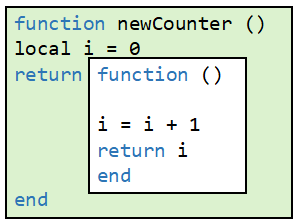
\includegraphics[scale=2.98, width=160pt, height=100pt]{zatvorenje.png}
\caption{Primer zatvorenja}
\end{figure}


\end{frame}


%--------------------------------------------------


\subsection{Iteratori}
\begin{frame}
\frametitle{Iteratori}

\begin{itemize}
\item Konstrukcije koje omogćuju prolazak kroz kolekciju
\item Iteratori sa stanjem
\begin{itemize}
\item Koriste zatvorenja kako bi zapamtili prethodno stanje u kom su bili
\item Čuvaju svoja stanja u okviru spoljašnje funkcije
\end{itemize}
\item Iteratori bez stanja
\begin{itemize}
\item Ne čuvaju sami svoja stanja
\item Isti iterator se može iskoristiti u više petlji, bez potrebe za pravljenjem novih zatvorenja
\end{itemize}
\end{itemize}

\end{frame}



\begin{frame}

\begin{block}{Primer iteratora sa stanjem}
\begin{semiverbatim}
function values ( t )

	\quad local i = 0
	
	\quad return function () i = i + 1; return t [ i ] end
	
end

t = \{10 , 20 , 30\}

for element in values ( t ) do

	\quad print ( element )
	
end
\end{semiverbatim}
\end{block}

\begin{block}{Primer iteratora bez stanja}
\begin{semiverbatim}
a = \{ " one " , " two " , " three " \}

for i , v in ipairs ( a ) do

	\quad print (i , v )

end

\end{semiverbatim}
\end{block}


\end{frame}

%--------------------------------------------------

\section{Zaključak}

\begin{frame}
\frametitle{Zaključak}

\begin{itemize}
\item Iako je nastala za lokalne potrebe, Lua danas ima primenu u svetu
\item Lua podržava objektno-orijentisanu, funkcionalnu i proceduralnu paradigmu
\item Lua raspolaže malim brojem mehanizama, ali efikasnim
\end{itemize}

\end{frame}

%------------------------------------------------

\section{Literatura}

\begin{frame}
\frametitle{Literatura}
\footnotesize{
\begin{thebibliography}{99}

\bibitem[]{p1} Roberto Ierusalimschy (2006)
\newblock \small{\textbf{Programming in Lua.} Lua.org, Rio de Janeiro, 2006.}

\bibitem[]{p1} Roberto Ierusalimschy (2003-2004)
\newblock \small{\textbf{Lua.org}, on-line at: https://www.lua.org/pil/7.1.html.}

\bibitem[]{p1} Etiene Dalcol (2014-2015)
\newblock \small{\textbf{Sailor Project}, on-line at: http://sailorproject.org/main/about.}

\end{thebibliography}
}
\end{frame}


\end{document} 
